\documentclass[conference]{IEEEtran}

\usepackage{cite}
\usepackage{amsmath,amssymb,amsfonts}
\usepackage{graphicx}
\usepackage{textcomp}
\usepackage{hyperref}
\usepackage{booktabs}
\usepackage{multirow}

\graphicspath{{figures/}}

\begin{document}

\title{MorphoCLIP: Text-Supervised Contrastive Learning for Perturbation Matching in Cell Painting Images}

\author{
  \IEEEauthorblockN{Sukhrobbek Ilyosbekov}
  \IEEEauthorblockA{
    Northeastern University \\
    Portland, ME, USA \\
    ilyosbekov.s@northeastern.edu
  }
  \and
  \IEEEauthorblockN{Shubham Gajjar}
  \IEEEauthorblockA{
    Northeastern University \\
    Portland, ME, USA \\
    gajjar.shu@northeastern.edu
  }
  \and
  \IEEEauthorblockN{Rongfei Jin}
  \IEEEauthorblockA{
    Northeastern University \\
    Portland, ME, USA \\
    jin.ron@northeastern.edu
  }
}

\maketitle

\begin{abstract}
  Cell Painting images record how cells respond to a chemical or genetic perturbation, and matching an image back to the perturbation that produced it is a basic step in phenotypic drug discovery that current methods still do poorly.
  We present MorphoCLIP, a contrastive model that places Cell Painting wells and text descriptions of perturbations in a shared 512-dimensional space. Each fluorescence channel passes through a frozen DINOv3 ViT-L/16, a one-layer CrossChannelFormer merges the five channel tokens, and a frozen BioClinical ModernBERT encodes the prompt; only the channel transformer and two projection heads are trained, about 14M parameters, and one model covers compounds, CRISPR knockouts and ORF overexpressions. With both backbones cached, an epoch over the CPJUMP1 pilot takes seconds on one 16\,GB GPU.
  Ranking held-out perturbation profiles against 98 candidate texts gives Recall@10 near 39\% in both directions on the validation split (random: 10\%), and 37\% image-to-text and 44\% text-to-image on the test split (random: 12\%).
  We add three terms to the training signal, a replicate-alignment image loss, gene-aware soft labels and per-plate offsets measured against replicate plates, and measure each alone. Their effect on retrieval is within the spread a single checkpoint shows between splits at one seed. The replicate loss does raise replicability on the standard CPJUMP1 benchmark on all twelve tracks (mean fraction retrieved 0.18 to 0.25, and 0.28 with all three additions), a gain that is partly definitional; plate offsets alone leave the benchmark unchanged.
  On the same harness, compound replicability is level with or above the released CellCLIP checkpoint at one hundredth of its size, and compound target matching falls inside the published CellProfiler range. Cross-modality gene--compound matching is at or near zero for every variant (at most three of 179 to 480 compound--gene pairs pass the significance gate), and we report that as an open failure.
  We also document an evaluation pitfall: ranking wells against a text pool in which each text appears once per replicate well caps recall and made image-to-text retrieval look worse than chance.
\end{abstract}

\begin{IEEEkeywords}
  contrastive learning, cell painting, morphological profiling, CLIP, perturbation matching
\end{IEEEkeywords}

\section{Introduction}

Phenotypic drug discovery asks how a chemical or genetic perturbation changes the state of a cell, at a scale that target-specific assays cannot reach. Bringing one drug to approval costs on the order of \$2\,B and takes about a decade~\cite{wouters2020rdcost}, while roughly nine of ten compounds that enter clinical trials fail~\cite{sun2022clinicaltrials}.

High-content microscopy is one way to get that scale. The Cell Painting assay~\cite{bray2016cellpainting, seal2024cellpainting} stains cells with five fluorescent dyes that mark DNA, endoplasmic reticulum, RNA and nucleoli, actin and Golgi, and mitochondria, and images them as a five-channel picture of cellular state. A perturbation changes that picture, and the change carries information about the perturbation's mechanism. The CPJUMP1 benchmark~\cite{chandrasekaran2024jump} turns this into a retrieval problem over about 3 million fields of view: given images of cells treated with 303 compounds, 160 CRISPR knockouts and 176 ORF overexpressions, can a model match perturbations that act on the same target?

Existing methods each cover part of this problem, and none covers all of it. The CellProfiler pipeline~\cite{carpenter2006cellprofiler} measures handcrafted features and recovers 5 to 25\% of the expected sister-perturbation matches on CPJUMP1~\cite{chandrasekaran2024jump}. CLOOME~\cite{sanchez2023cloome} and MolPhenix~\cite{fradkin2024molphenix} learn contrastive image encoders against molecular fingerprints, and so handle compounds only. CellCLIP~\cite{lu2025cellclip} replaces fingerprints with text prompts, which admits genetic perturbations, but runs on a 1.48B-parameter DINOv2-g stack and its cross-class retrieval trails CellProfiler. CWA-MSN~\cite{huang2025cwamsn} attacks batch effects directly and beats CellCLIP on gene--gene retrieval with 22M parameters, but has no text branch and cannot be queried in language.

MorphoCLIP combines text supervision, joint training over compounds and genes, and a batch-correction option in one model. It follows CLIP~\cite{radford2021clip}: an image encoder and a text encoder are trained so that a Cell Painting well and the description of its perturbation land close together in a shared 512-dimensional space. Both backbones are frozen and their outputs are cached. The trainable components are a one-layer transformer over channel tokens, two projection heads and one logit-scale scalar, about 14M parameters in total, compared with CellCLIP's 1.48B total parameters.

The paper makes four contributions.
\begin{enumerate}
    \item A text-supervised model over cached DINOv3 channel tokens~\cite{simeoni2025dinov3}, trained jointly on compounds, CRISPR knockouts and ORF overexpressions with two frozen backbones.
    \item Three additions measured separately against a shared control: an image--image replicate loss, gene-aware soft labels, and a per-plate offset relative to replicate plates of the same condition. The replicate loss increases deterministic replicability mAP on every benchmark track; retrieval differences and the other additions remain unresolved at one seed.
    \item Perturbation-level retrieval with analytic random baselines and evaluation on the standard CPJUMP1 benchmark. Separate stochastic benchmark runs show numerically comparable compound replicability fractions for MorphoCLIP and the released CellCLIP checkpoint, without supporting a ranking. The four-track mean compound target-matching fraction lies within the published CellProfiler range, although one track is above it. Gene--compound fraction retrieved remains at or near zero.
    \item A documented evaluation pitfall: duplicating each text once per replicate well creates tied blocks of candidates, caps Recall@5 and Recall@10 near Recall@1, and invalidates a shuffled-well baseline for image-to-text retrieval.
\end{enumerate}

\section{Problem Statement}

Given a five-channel Cell Painting image $\mathbf{x} \in \mathbb{R}^{5 \times H \times W}$ and a
text description $t$ of the applied perturbation, we learn image and text encoders that map both
inputs to the same normalized embedding space:
\begin{equation}
  f_{\text{img}}(\mathbf{x}),\;
  f_{\text{txt}}(t) \in \mathbb{R}^d,
  \quad
  \|f_{\text{img}}(\mathbf{x})\|_2
  = \|f_{\text{txt}}(t)\|_2
  = 1.
\end{equation}
Matching image--text pairs should have high cosine similarity, while unrelated pairs should be
farther apart. We set $d=512$. Although the equation is written for one image, the model operates
at the well level by combining all imaged sites from a well into one vector.

The trained encoders support three retrieval tasks:
\begin{itemize}
  \item \textbf{Text-to-image retrieval.}
        Given a perturbation description, retrieve the wells that show the corresponding phenotype.
  \item \textbf{Image-to-text retrieval.}
        Given a well, return the perturbation description that best matches its morphology.
  \item \textbf{Image-to-image retrieval.}
        Compare well embeddings by cosine similarity, without text at inference time. This is the
        setting of the standard CPJUMP1 benchmark: do replicate wells of one perturbation match, and
        do perturbations that share a target match across modalities?
\end{itemize}

This task is harder than ordinary image--caption alignment for three reasons.

\paragraph{Batch effects.}
The same perturbation can look different across plates and imaging days. Changes in illumination,
staining or focus may be stronger than the biological effect of interest. In CPJUMP1,
reproducibility also varies by perturbation type and cell line~\cite{chandrasekaran2024jump}.

\paragraph{Imperfect labels.}
Biological similarity is not simply positive or negative. Two compounds may share a primary target
but differ in their secondary effects, while a gene knockout and a compound may influence the same
pathway through different mechanisms. This motivates softer supervision than a standard loss in
which every non-matching pair is treated as equally negative.

\paragraph{Scale and compute.}
CPJUMP1 contains several terabytes of microscopy data. Training both foundation models end to end
is impractical on a single consumer GPU, so we run the frozen backbones once, cache their outputs
and train only the smaller modules on top.

\section{Related Work}

\subsection{Morphological Profiling}

Cell Painting~\cite{bray2016cellpainting} established the five-stain assay now widely used for high-content morphological profiling~\cite{seal2024cellpainting}. The standard analysis pipeline, CellProfiler~\cite{carpenter2006cellprofiler}, measures more than a thousand handcrafted properties of each cell. These features remain a strong baseline on CPJUMP1~\cite{chandrasekaran2024jump}, although matching compounds to genetic perturbations is still difficult.

Handcrafted pipelines are limited to a predefined set of measurements. Self-supervised vision transformers have shown stronger transfer on drug-target and gene-family classification~\cite{moshkov2025ssl}, which motivates our use of frozen foundation-model features.

\subsection{Contrastive Learning for Cell Painting}

CLOOME~\cite{sanchez2023cloome} introduced CLIP-style training for Cell Painting by pairing a ResNet image encoder with molecular fingerprints. Its compound retrieval results showed that contrastive supervision works for Cell Painting, but the method does not cover genetic perturbations and treats the five fluorescence channels as RGB.

MolPhenix~\cite{fradkin2024molphenix} uses a frozen Phenom-1 image encoder, averages replicate embeddings and introduces softer labels. It improves compound retrieval but depends on a proprietary backbone and likewise does not represent genetic perturbations.

CellCLIP~\cite{lu2025cellclip} is the closest prior work. It combines templated text prompts with per-channel image encoding, cross-channel attention, attention-based cell pooling and a continuously weighted contrastive loss. Its text branch can describe chemical and genetic perturbations in a common form. However, it relies on a much larger DINOv2-g backbone, and its cross-class results show that text supervision alone does not solve technical variation between experiments.

\subsection{Batch-Effect Correction}

CWA-MSN~\cite{huang2025cwamsn} addresses batch effects within a masked Siamese network by aligning cells that received the same perturbation across wells and plates. This improves gene--gene retrieval without relying on explicit batch labels. The model has no text branch, but its alignment strategy is closely related to the replicate loss studied here.

\subsection{Foundation Models for Microscopy}

DINOv2~\cite{oquab2024dinov2} and DINOv3~\cite{simeoni2025dinov3} give self-supervised visual features that transfer to biological imaging despite natural-image pretraining~\cite{moshkov2025ssl}. DINOv3 adds gram anchoring and a revised training recipe. Channel Vision Transformers~\cite{bao2024channelvit} show that per-channel encoding followed by cross-channel attention works for multi-channel microscopy, which is the pattern our channel aggregator follows.

On the text side, BioClinical ModernBERT~\cite{sounack2025bioclinical} is pretrained on biomedical and clinical literature. A single model can encode both small-molecule and gene descriptions, unlike encoders designed only for chemical strings. This makes it a natural fit for a dataset that mixes compounds with genetic perturbations.

\subsection{Positioning of MorphoCLIP}

Table~\ref{tab:methods} places MorphoCLIP among these methods. CellCLIP has text but no batch correction. CWA-MSN has batch correction but no text. MorphoCLIP has both, trains on all three perturbation types, and keeps the trained part small. Where a like-for-like number exists we compare on the same benchmark harness (Section~\ref{sec:results}); elsewhere we quote published figures and say what differs.

\begin{table}[t]
\centering
\caption{Cell Painting representation learning methods. The parameter count is trainable parameters for MorphoCLIP and total parameters for the other learned methods.}
\label{tab:methods}
\resizebox{\columnwidth}{!}{%
\begin{tabular}{@{}lccccc@{}}
\toprule
Method & Image Encoder & Text & Pert.\ Types & Batch Corr.\ & Params \\
\midrule
CellProfiler~\cite{carpenter2006cellprofiler} & Handcrafted & No & All & Sphering & N/A \\
CLOOME~\cite{sanchez2023cloome} & ResNet & No & Compounds & No & ${\sim}$25M \\
MolPhenix~\cite{fradkin2024molphenix} & Phenom-1 & No & Compounds & No & ${\sim}$36M \\
CellCLIP~\cite{lu2025cellclip} & DINOv2-g & Yes & All & No & 1,477M \\
CWA-MSN~\cite{huang2025cwamsn} & ViT-S/16 & No & Unimodal & CWA & 22M \\
\textbf{MorphoCLIP} & DINOv3-L & Yes & All & Plate offsets & ${\sim}$14M \\
\bottomrule
\end{tabular}%
}
\end{table}

\section{Method}

MorphoCLIP has image and text encoders trained with a contrastive text objective and optional replicate and plate-offset terms. The image encoder turns a well of five-channel Cell Painting sites into a 512-dimensional unit vector. The text encoder does the same for a prompt that describes the perturbation. Figure~\ref{fig:architecture} shows the pipeline.

\begin{figure*}[t]
    \centering
    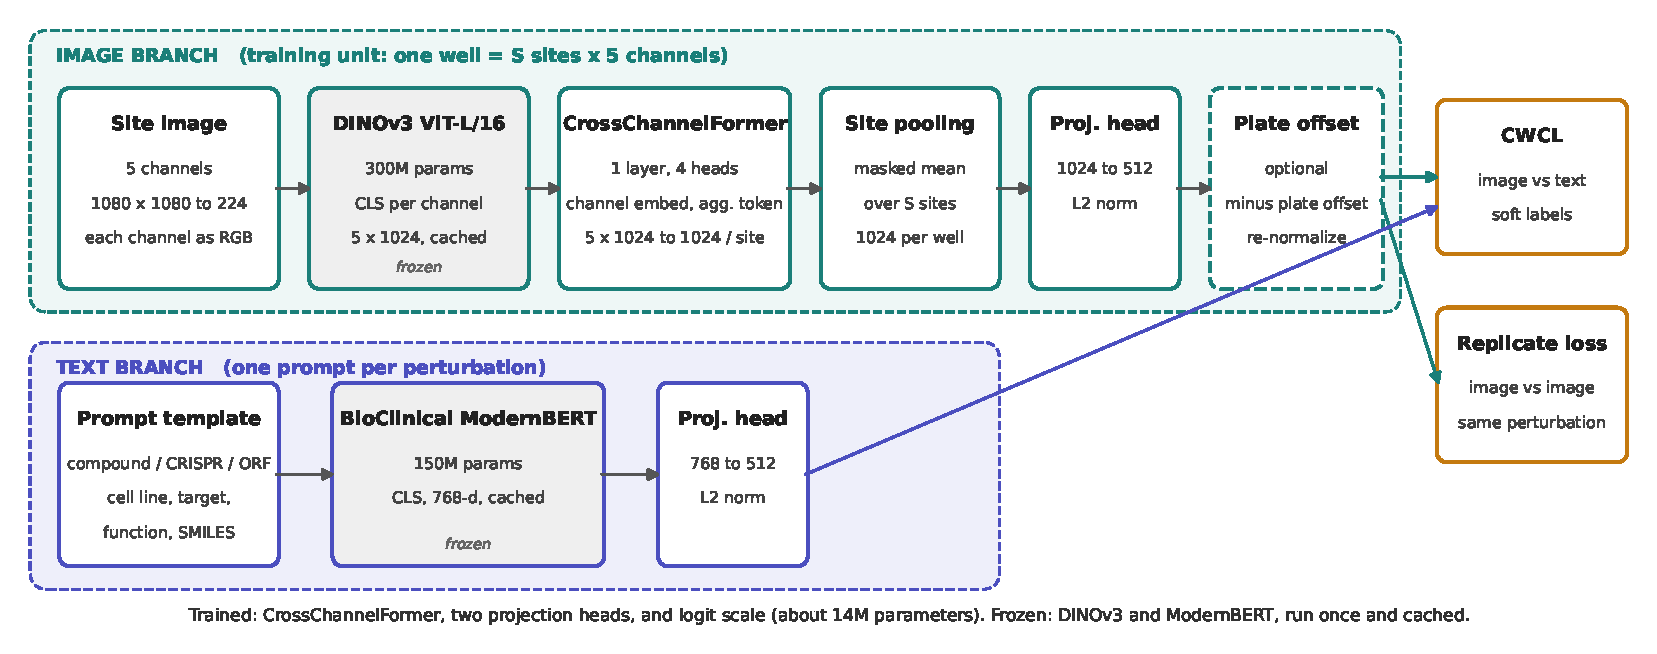
\includegraphics[width=\textwidth]{figures/architecture.pdf}
    \caption{MorphoCLIP. Each fluorescence channel of a site is encoded on its own by a frozen DINOv3 ViT-L/16, giving five 1024-d CLS tokens. A one-layer CrossChannelFormer attends over the five channel tokens and a learned aggregation token, and the aggregation token's output is the site vector. Site vectors are mean-pooled into a well vector and projected to the shared 512-d space. The prompt is encoded by a frozen BioClinical ModernBERT and projected to the same space. When plate offsets are on, the image embedding is shifted by its plate's offset and re-normalized before the losses. The trainable components are the CrossChannelFormer, the two projection heads and one logit-scale scalar, about 14M parameters in total.}
    \label{fig:architecture}
\end{figure*}

\subsection{Image Encoder}

A Cell Painting site has five fluorescence channels (Table~\ref{tab:channels}). We encode each channel on its own: the single-channel image is resized to the Hugging Face processor's native $224 \times 224$ input, copied to three channels, normalized with the processor statistics, and passed through a frozen DINOv3 ViT-L/16~\cite{simeoni2025dinov3} (300M parameters). The result is five 1024-dimensional CLS tokens per site,
\begin{equation}
    \{\mathbf{z}_c\}_{c=1}^{5}, \quad \mathbf{z}_c \in \mathbb{R}^{1024}.
\end{equation}

\begin{table}[t]
\centering
\caption{Cell Painting fluorescence channels used in MorphoCLIP.}
\label{tab:channels}
\begin{tabular}{@{}cll@{}}
\toprule
Ch & Stain & Target \\
\midrule
1 & MitoTracker / Alexa 647 & Mitochondria \\
2 & Phalloidin / Alexa 568 & Actin \\
3 & WGA / Alexa 488 & Golgi / plasma membrane \\
4 & Concanavalin A / Alexa 488 & Endoplasmic reticulum \\
5 & Hoechst 33342 & DNA / nucleus \\
\bottomrule
\end{tabular}
\end{table}

We use DINOv3 ViT-L rather than the larger DINOv2-g backbone used by CellCLIP. The channel tokens are written to disk once, and every training run reads from that cache. The backbone never runs during training.

\paragraph{CrossChannelFormer (CCF).} A one-layer transformer encoder~\cite{vaswani2017attention} with 4 heads merges the five channel tokens into one site vector, following the channel-aware design of CellCLIP~\cite{lu2025cellclip} and Channel ViT~\cite{bao2024channelvit}. Each token is L2-normalized so the five channels enter at a common scale, then a learned channel embedding $\mathbf{e}_c$ is added so the transformer can tell the stains apart. A learned aggregation token $\mathbf{q}$ is prepended and its output is the site vector:
\begin{equation}
    \mathbf{h}_{\text{site}} = \bigl[\,\text{CCF}\bigl(\mathbf{q},\, \hat{\mathbf{z}}_1 + \mathbf{e}_1,\, \dots,\, \hat{\mathbf{z}}_5 + \mathbf{e}_5\bigr)\,\bigr]_{0}, \quad \hat{\mathbf{z}}_c = \mathbf{z}_c / \|\mathbf{z}_c\|_2 .
\end{equation}
The layer is pre-norm with a feed-forward width of 4096 and GELU activations. The transformer can read out joint patterns across stains, for example a change that shows in both the mitochondrial and the ER channel. The CCF holds 12.6M of the 14M trained parameters.

\paragraph{Site-to-well pooling.} The training unit is a well. Site vectors are averaged under a site mask, so wells with 7, 9 or 16 imaged sites all produce one vector and the order of sites does not matter.

\paragraph{Image projection head.} A two-layer MLP with LayerNorm, GELU and dropout ($p = 0.3$) maps the well vector $\mathbf{h}_{\text{img}}$ to the shared space:
\begin{equation}
    f_{\text{img}}(\mathbf{x}) = \text{L2Norm}\bigl(\mathbf{W}_2\, \text{Drop}(\text{GELU}(\text{LN}(\mathbf{W}_1 \mathbf{h}_{\text{img}})))\bigr),
\end{equation}
with $\mathbf{W}_1 \in \mathbb{R}^{512 \times 1024}$ and $\mathbf{W}_2 \in \mathbb{R}^{512 \times 512}$.

\subsection{Text Encoder}

Each perturbation gets one prompt, built from CPJUMP1 metadata and external annotations with one of four templates:

\begin{itemize}
    \item \textbf{Compound:} \textit{``Cell Painting morphological profile of \{cell\_line\} cells treated with the compound \{compound\_name\}. Chemical structure (SMILES): \{smiles\}. Known target gene: \{target\_gene\}. Target protein function: \{gene\_function\}. Perturbation modality: chemical compound.''}
    \item \textbf{CRISPR:} \textit{``\dots\ with CRISPR-Cas9 knockout of gene \{gene\_symbol\}. Gene description: \{gene\_description\}. Gene function: \{gene\_function\}. Perturbation modality: CRISPR knockout.''}
    \item \textbf{ORF:} \textit{``\dots\ overexpressing gene \{gene\_symbol\} via open reading frame construct. Gene description: \{gene\_description\}. Gene function: \{gene\_function\}. Perturbation modality: ORF overexpression.''}
    \item \textbf{Negative control:} \textit{``\dots\ treated with DMSO vehicle control. No active perturbation applied.''}
\end{itemize}

Missing fields become ``unknown''. Compound annotations come from ChEMBL and the CPJUMP1 metadata. Gene descriptions and functions come from UniProt. Prompts are keyed by the perturbation identifier (\texttt{broad\_sample}), so replicate wells of one perturbation share one text vector.

We encode each prompt with a frozen BioClinical ModernBERT~\cite{sounack2025bioclinical} (150M parameters, 768-d CLS token). A trainable projection head with the same shape as the image head maps the CLS token to the shared space:
\begin{equation}
    f_{\text{txt}}(t) = \text{L2Norm}\bigl(\mathbf{W}_4\, \text{Drop}(\text{GELU}(\text{LN}(\mathbf{W}_3 \mathbf{h}_{\text{txt}})))\bigr),
\end{equation}
with $\mathbf{W}_3 \in \mathbb{R}^{512 \times 768}$ and $\mathbf{W}_4 \in \mathbb{R}^{512 \times 512}$. The 768-d BERT outputs are cached separately from the projected 512-d vectors, so a change to the projection head never re-runs BERT.

\subsection{Training Objective}

\paragraph{Continuously weighted contrastive loss (CWCL).} InfoNCE~\cite{oord2018infonce} treats every off-diagonal pair in a batch as a negative. That is wrong when two wells in the batch carry the same perturbation, and questionable when two compounds share a target. Following CellCLIP~\cite{lu2025cellclip}, we use a soft-label variant. For a batch of $N$ wells with logits $\mathbf{S} = \tau\, \mathbf{F}_{\text{img}} \mathbf{F}_{\text{txt}}^{\top}$, an affinity matrix $\mathbf{W} \in [0,1]^{N \times N}$ sets $w_{ij} = 1$ when wells $i$ and $j$ carry the same perturbation, $w_{ij} = \alpha$ when their perturbations differ but their target-gene sets overlap, and $w_{ij} = 0$ otherwise. The loss is
\begin{equation}
    \mathcal{L}_{\text{CWCL}} = -\frac{1}{2N} \sum_{i=1}^{N} \sum_{j=1}^{N} \Bigl( \tilde{w}_{ij} \log p_{ij} + \tilde{w}^{\top}_{ij} \log p^{\top}_{ij} \Bigr),
\end{equation}
where $p_{ij}$ is the softmax of row $i$ of $\mathbf{S}$, $\tilde{w}_{ij} = w_{ij} / \sum_k w_{ik}$, and the transposed terms use $\mathbf{S}^{\top}$ and $\mathbf{W}^{\top}$ normalized over their own rows. The gene weight $\alpha$ is a hyperparameter; the base model uses $\alpha = 0$ (binary labels) and the soft-label ablation uses $\alpha = 0.6$. The scale $\tau$ is learned through its logarithm, which starts at $\ln(1/0.07)$ and is clamped to $[0, \ln 100]$ after every step.

\paragraph{Replicate alignment loss.} The text loss never asks two replicate wells of one perturbation to be near each other. It only asks each to be near their shared text. We add an image--image term that does. With $P_i$ the set of other wells in the batch that carry the same perturbation as well $i$ and $\mathbf{G} = \tau\, \mathbf{F}_{\text{img}} \mathbf{F}_{\text{img}}^{\top}$ with the diagonal masked out,
\begin{equation}
    \mathcal{L}_{\text{rep}} = -\frac{1}{|\{i : P_i \neq \emptyset\}|} \sum_{i:\, P_i \neq \emptyset} \frac{1}{|P_i|} \sum_{j \in P_i} \log \frac{\exp G_{ij}}{\sum_{k \neq i} \exp G_{ik}} .
\end{equation}
Wells with no in-batch replicate are dropped from the mean, and the term shares the learned temperature with the text loss. The training loss is $\mathcal{L} = \mathcal{L}_{\text{CWCL}} + \lambda_{\text{rep}} \mathcal{L}_{\text{rep}}$; the base model uses $\lambda_{\text{rep}} = 0$ and the ablation uses $0.3$. Validation loss is the text term alone, so model selection is not influenced by the added term.

\paragraph{Perturbation-aware batches.} For the replicate term to have positives, replicate wells must share a batch. Our sampler groups the training wells by perturbation, cuts each group into chunks of two wells, shuffles the chunks and packs them into batches of 256. A repair pass swaps chunks so that every batch spans at least two plates where possible. This is a batch-composition constraint; it does not guarantee that individual negative pairs are free of plate confounding. Every ablation run uses this sampler; the base model uses uniform random batches.

\paragraph{Plate offsets (cross-well alignment).} Batch effects are the main confound in Cell Painting, but in CPJUMP1 a plate is close to synonymous with an experimental condition (one cell line, one perturbation modality, one timepoint). Subtracting a plate's mean embedding would therefore also subtract the condition, which is exactly what the prompt describes. Our correction is relative to replicate plates instead. At the start of each epoch a gradient-free pass over the training wells computes each plate's mean embedding $\bar{\mathbf{f}}_p$, and every well is shifted by its plate's offset from the mean of the plates in the same condition:
\begin{equation}
    \tilde{\mathbf{f}}_w = \frac{\mathbf{f}_w - \boldsymbol{\delta}_{p(w)}}{\|\mathbf{f}_w - \boldsymbol{\delta}_{p(w)}\|_2}, \quad \boldsymbol{\delta}_p = \bar{\mathbf{f}}_p - \frac{1}{|C(p)|} \sum_{q \in C(p)} \bar{\mathbf{f}}_q ,
\end{equation}
where $p(w)$ is the plate of well $w$ and $C(p)$ is the set of plates that share plate $p$'s condition. Offsets within a condition sum to zero, so the step removes replicate-to-replicate drift and cannot remove the condition itself. The condition of each plate comes from the CPJUMP1 reference metadata; the eleven plates that the reference table does not cover (non-standard seeding density, antibiotics, or compounds on the Cas9 line) are keyed on every condition axis from the experiment table so they are not merged into a standard group. Offsets are constants (no gradient flows through them), apply to image embeddings only, are frozen within an epoch, and are stored in the checkpoint so evaluation and profile export apply the same correction as training. An earlier version of this component subtracted the in-batch plate mean instead. It removed the condition signal and cut retrieval to near chance; Section~\ref{sec:results} reports that run for completeness.

\subsection{Optimization}

We train with AdamW~\cite{loshchilov2019adamw} at learning rate $10^{-4}$, $(\beta_1, \beta_2) = (0.9, 0.999)$ and $\varepsilon = 10^{-8}$. Weight decay 0.2 is applied to parameters with at least two dimensions except parameters whose names identify biases or normalization layers; it is not applied to one-dimensional parameters or the learned temperature. The learning rate warms up linearly for 100 steps and then follows a cosine schedule to zero. We use FP16 mixed precision, gradient clipping at norm $1.0$ and a batch of 256 wells. The base model trained on a 100-epoch schedule and its best validation loss came at epoch 9; the ablation runs use a 30-epoch schedule with early stopping after 8 epochs without improvement. The recorded \texttt{epoch\_seconds} is about four seconds for 55 optimizer steps on an RTX 5080 with the cache in RAM. That timer excludes validation and, for offset runs, the gradient-free offset refresh, so it is not end-to-end epoch or run time.

\section{Experimental Setup}

\subsection{Dataset}

We use the CPJUMP1 pilot~\cite{chandrasekaran2024jump}, a public dataset from the JUMP Cell
Painting Consortium. It contains 303 small-molecule compounds, 160 CRISPR knockouts and 176 ORF
overexpressions measured in U2OS and A549 cells. Most perturbation types were collected at two
timepoints. Each well contains several imaged sites with five fluorescence channels; the three
available brightfield channels are not used in this study.

\subsection{Data Pipeline}

Because the raw images occupy several terabytes, we process one plate at a time. After DINOv3
produces the per-channel features, the raw local copy is removed and the cached features are reused
in every training run. Text prompts are handled similarly: ModernBERT encodes each prompt once, and
the resulting feature is stored for later training.

\subsection{Splits}

We split the data by perturbation rather than by well. A fixed hash assigns each perturbation to
the training, validation or test set in an 80/10/10 ratio, so replicate wells of one perturbation
never appear in different splits. All three perturbation types are represented in each split, and
control wells are excluded from training and retrieval evaluation. The validation set contains
2,220 wells from 98 perturbations, and the test set contains 1,860 wells from 86 perturbations.

\subsection{Retrieval Protocol}
\label{sec:protocol}

Replicate wells share a text description. A split therefore contains $P$ distinct text vectors and
$N$ well vectors. We evaluate four retrieval settings and compute an analytic chance baseline for
each one.

\begin{itemize}
  \item \textbf{Well-level image-to-text.}
        Each of the $N$ wells ranks the $P$ unique texts. One candidate is correct. Random
        Recall@$k$
        is $k/P$.
  \item \textbf{Well-level text-to-image.}
        Each of the $P$ texts ranks all $N$ wells and is scored on the rank of its first correct
        replicate. With $m$ replicate wells among $N$ candidates, random Recall@$k$ is
        $1 - \binom{N-m}{k} / \binom{N}{k}$.
  \item \textbf{Perturbation-level, both directions.}
        The well embeddings of each perturbation are averaged and re-normalized into one profile,
        and the $P$ profiles are ranked against the $P$ texts. This is the unit of the standard
        CPJUMP1 protocol. Random Recall@$k$ is $k/P$.
\end{itemize}
We report Recall@\{1, 5, 10\} and the median rank of the first correct match. Checkpoints are
selected using validation text loss and then evaluated on both validation and test data.

\subsection{Standard CPJUMP1 Benchmark}

We also evaluate exported well embeddings with the standard CPJUMP1 benchmark of Chandrasekaran et
al.~\cite{chandrasekaran2024jump}. We follow the reference pipeline: every well is encoded in fp32,
including controls, and the negative-control mean is removed before scoring. The benchmark uses the
40 plates that meet its standard experimental criteria and covers a short and long timepoint for
each perturbation type. It measures \emph{replicability} between repeated wells, \emph{target
  matching} between perturbations of the same type and \emph{gene--compound matching} across
perturbation types. Results are reported as mean average precision (mAP) and as the fraction of
perturbations that pass the benchmark's significance threshold.

The benchmark's significance test uses random permutations, so fraction retrieved varies slightly
between otherwise identical runs. Replicability mAP is deterministic. We therefore treat small
differences in fraction retrieved as descriptive rather than conclusive.

\subsection{Baselines}

\begin{itemize}
  \item \textbf{CellProfiler}~\cite{carpenter2006cellprofiler} provides the established
        handcrafted-feature baseline. We use its published CPJUMP1 target-matching range because we
        did not rerun the full pipeline.
  \item \textbf{CellCLIP}~\cite{lu2025cellclip} is the closest text-supervised baseline. We report
        its published results and also run the released checkpoint through our short-timepoint
        benchmark pipeline. This comparison is approximate because CellCLIP applies an additional
        KernelPCA correction and the benchmark significance test is stochastic.
  \item \textbf{CWA-MSN}~\cite{huang2025cwamsn} is included as a related batch-aware method. Its
        published benchmarks differ from ours, so a direct numerical comparison is not possible.
\end{itemize}

\subsection{Ablation Design}
\label{sec:ablation_design}

The base model uses binary CWCL labels, random batches, no replicate loss and no plate correction.
The ablations use perturbation-aware batches, a shorter schedule and early stopping. Starting from
this shared control, we add gene-aware soft labels ($\alpha=0.6$), replicate alignment
($\lambda_{\text{rep}}=0.3$) and condition-relative plate offsets one at a time, followed by a run
that combines all three. All runs use seed 42, batch size 256 and the same data split. Since a
single retrieved perturbation changes recall by about one percentage point, small differences
should not be interpreted as reliable effects.

\subsection{Implementation}

All experiments run on one RTX 5080 with 16\,GB of memory. We use AdamW with a learning rate of
$10^{-4}$, weight decay of 0.2, 100 warm-up steps followed by cosine decay, FP16 training and
gradient clipping at 1.0. The CrossChannelFormer has one layer and four attention heads; both
projection heads use a hidden width of 512 and dropout of 0.3. Code, configurations and split
manifests are released with the paper.

\section{Results and Discussion}
\label{sec:results}

All numbers come from a single seed. Retrieval numbers are on the validation and test splits described in Section~\ref{sec:protocol}; benchmark numbers are on the 40 benchmark-eligible plates. We give the random baseline next to every retrieval figure and note where a difference is smaller than one perturbation's worth of recall.

\subsection{Cross-Modal Retrieval}

Table~\ref{tab:retrieval} reports the base model on both splits. On validation, ranking the 98 perturbation profiles against the 98 texts gives Recall@10 of 38.8\% image-to-text and 39.8\% text-to-image, against a random 10.2\%, with a median rank of 13. On the 86 test perturbations the same checkpoint gives 37.2\% and 44.2\% against a random 11.6\%. These recalls are 3.2 to 3.9 times their analytic chance rates.

\begin{table}[t]
\centering
\caption{Retrieval of the base model on the validation split (2,220 wells, 98 perturbations) and the test split (1,860 wells, 86 perturbations). Well-level image-to-text ranks the unique texts; well-level text-to-image ranks all wells and scores the first correct replicate; perturbation-level ranks mean profiles against texts. Random rows are analytic. Median rank is over the candidate pool of each direction ($P$ texts, $N$ wells, or $P$ profiles).}
\label{tab:retrieval}
\resizebox{\columnwidth}{!}{%
\begin{tabular}{@{}llrrrr@{}}
\toprule
Split & Direction & R@1 & R@5 & R@10 & Med.\ rank \\
\midrule
\multirow{6}{*}{Val}
 & well image $\to$ text & 5.9 & 23.3 & 39.4 & 14 \\
 & well text $\to$ image & 4.1 & 15.3 & 23.5 & 30 \\
 & pert.\ image $\to$ text & 4.1 & 20.4 & 38.8 & 13 \\
 & pert.\ text $\to$ image & 5.1 & 18.4 & 39.8 & 13 \\
 & random, single positive & 1.0 & 5.1 & 10.2 & 49.5 \\
 & random, well text $\to$ image & 1.0 & 5.0 & 9.7 & 99 \\
\midrule
\multirow{6}{*}{Test}
 & well image $\to$ text & 5.5 & 22.0 & 41.4 & 13 \\
 & well text $\to$ image & 4.7 & 18.6 & 26.7 & 25 \\
 & pert.\ image $\to$ text & 4.7 & 17.4 & 37.2 & 14 \\
 & pert.\ text $\to$ image & 8.1 & 23.3 & 44.2 & 13 \\
 & random, single positive & 1.2 & 5.8 & 11.6 & 43.5 \\
 & random, well text $\to$ image & 1.2 & 5.7 & 11.0 & 86 \\
\bottomrule
\end{tabular}%
}
\end{table}

Well-level text-to-image is the one direction that looks weak in Recall@10 (23.5\% against 9.7\%), but that metric asks the text to place one of its 24 replicate wells in the top ten of 2,220, and its median rank of 30 says the first replicate is usually found within the top 1.4\% of the pool. Once wells are averaged into profiles the two directions agree.

\subsection{Ablations}

Table~\ref{tab:ablation} lists the single-factor runs.

\begin{table*}[t]
\centering
\caption{Single-factor ablations from a shared control (perturbation-aware batches, 30-epoch schedule, early stopping, seed 42). Perturbation-level Recall@10 in percent, median rank over $P$ texts, on validation (98 perturbations) and test (86). Random Recall@10 is 10.2 on validation and 11.6 on test. One perturbation is about one point. Best epoch is the epoch selected by validation text loss.}
\label{tab:ablation}
\resizebox{\textwidth}{!}{%
\begin{tabular}{@{}llrrrrrrr@{}}
\toprule
 & & \multicolumn{3}{c}{Validation} & \multicolumn{3}{c}{Test} & \\
\cmidrule(lr){3-5} \cmidrule(lr){6-8}
Run & Change from control & i$\to$t & t$\to$i & Med. & i$\to$t & t$\to$i & Med. & Best ep. \\
\midrule
Base model & 100-epoch schedule, random batches & 38.8 & 39.8 & 13 & 37.2 & 44.2 & 14 & 9 \\
Control & none & 37.8 & 37.8 & 13 & 50.0 & 41.9 & 10 & 11 \\
Soft labels & $\alpha = 0.6$ & 37.8 & 42.9 & 14 & 44.2 & 47.7 & 12 & 13 \\
Replicate loss & $\lambda_{\text{rep}} = 0.3$ & 44.9 & 41.8 & 13 & 47.7 & 46.5 & 12 & 7 \\
Plate offsets (in-batch, removed) & \texttt{use\_cwa} & 15.3 & 10.2 & 45 & -- & -- & -- & 4 \\
Plate offsets (40 of 51 plates) & \texttt{use\_cwa} & 36.7 & 39.8 & 13 & -- & -- & -- & 8 \\
Plate offsets (all 51 plates) & \texttt{use\_cwa} & 41.8 & 38.8 & 13 & 41.9 & 43.0 & 12 & 7 \\
All three & soft $+$ replicate $+$ offsets & 42.9 & 43.9 & 13 & 46.5 & 45.3 & 11 & 9 \\
\bottomrule
\end{tabular}%
}
\end{table*}

The retrieval differences among the three additions are unresolved at one seed. The ordering changes on the test split, and changes of several percentage points represent only a few perturbations. We therefore do not claim a retrieval gain for any single addition. The replicate-loss checkpoint is selected at epoch 7 and the control at epoch 11, but one run per condition does not establish a difference in convergence rate.

The in-batch offset version yields perturbation-level image-to-text Recall@10 of 15.3\%, compared with 37.8\% for its control, and its best checkpoint occurs at epoch 4. Evaluating that checkpoint with correction disabled at inference gives 12\%, so the degradation arose during training. In CPJUMP1 a plate is nearly one condition, and the plate mean carries modality and cell-line information named by the prompt. The condition-relative offset avoids this degradation. Extending the condition map from 40 to all 51 plates changes validation image-to-text recall by five perturbations, which remains unresolved at one seed.

The combined run is among the higher-scoring rows on both splits but is not uniformly best. Its best validation text loss is 5.396, compared with 5.438 for the control. These single-seed results show that the three additions can be trained together; they do not establish an additive retrieval benefit.

\subsection{Standard CPJUMP1 Benchmark}

Table~\ref{tab:benchmark} reports fraction retrieved and mAP on the standard benchmark for the base model, the replicate-loss run, the plate-offset run and the combined run.

\begin{table*}[t]
\centering
\caption{Standard CPJUMP1 benchmark on the 40 eligible plates. Per-track rows give fraction retrieved at $q<0.05$ with track mAP in parentheses. Summary fractions are unweighted means over tracks; parenthetical summary mAP is pooled over the scored rows and is weighted by track size. Fraction retrieved varies between identical runs; only replicability mAP is deterministic.}
\label{tab:benchmark}
\begin{tabular}{@{}llrrrr@{}}
\toprule
Track & & Base & Replicate loss & Plate offsets & All three \\
\midrule
\multirow{2}{*}{Compound A549} & short & 0.353 (0.392) & 0.435 (0.458) & 0.327 (0.384) & 0.497 (0.493) \\
 & long & 0.513 (0.526) & 0.650 (0.583) & 0.503 (0.513) & 0.703 (0.626) \\
\multirow{2}{*}{Compound U2OS} & short & 0.297 (0.344) & 0.379 (0.404) & 0.310 (0.351) & 0.422 (0.439) \\
 & long & 0.369 (0.413) & 0.471 (0.474) & 0.395 (0.421) & 0.503 (0.496) \\
\multirow{2}{*}{CRISPR A549} & short & 0.173 (0.286) & 0.271 (0.343) & 0.092 (0.239) & 0.340 (0.375) \\
 & long & 0.183 (0.296) & 0.376 (0.356) & 0.134 (0.282) & 0.366 (0.385) \\
\multirow{2}{*}{CRISPR U2OS} & short & 0.026 (0.175) & 0.049 (0.207) & 0.052 (0.182) & 0.078 (0.232) \\
 & long & 0.170 (0.277) & 0.219 (0.290) & 0.160 (0.259) & 0.258 (0.318) \\
\multirow{2}{*}{ORF A549} & short & 0.006 (0.136) & 0.012 (0.158) & 0.012 (0.138) & 0.019 (0.174) \\
 & long & 0.000 (0.128) & 0.006 (0.142) & 0.000 (0.126) & 0.006 (0.141) \\
\multirow{2}{*}{ORF U2OS} & short & 0.043 (0.171) & 0.099 (0.223) & 0.062 (0.209) & 0.099 (0.221) \\
 & long & 0.006 (0.133) & 0.012 (0.146) & 0.012 (0.140) & 0.031 (0.160) \\
\midrule
Replicability summary (12 tracks) & & 0.178 (0.298) & 0.248 (0.343) & 0.172 (0.292) & 0.277 (0.369) \\
Target-matching summary (8 tracks) & & 0.339 (0.197) & 0.262 (0.160) & 0.420 (0.194) & 0.172 (0.148) \\
Gene--compound summary & & 0.005 (0.123) & 0.000 (0.082) & 0.010 (0.140) & 0.029 (0.082) \\
\bottomrule
\end{tabular}
\end{table*}

\paragraph{Replicability.} The replicate loss increases mAP on all twelve tracks; pooled mAP rises from 0.298 to 0.343. This deterministic metric is the clearest change in the study. It is also partly definitional: the loss pulls replicate wells of one perturbation together, and replicability measures whether those wells retrieve one another. The result shows that the loss achieves its direct objective, not that the embedding is more biologically informative. Plate offsets alone give pooled mAP 0.292. The combined run has pooled mAP 0.369 and exceeds the replicate-loss run on ten tracks while being slightly lower on two ORF tracks. Fraction-retrieved values are descriptive because their significance gate is stochastic.

\paragraph{Target matching.} The scored population changes with the replicability gate: the base, replicate-loss and combined runs admit 536, 748 and 856 consensus profiles. The CRISPR tracks contain only 2 to 30 targets, so their stochastic fractions move in large steps. Across the larger compound tracks, no variant is consistently ahead in mAP. The target-matching rows therefore do not establish a downstream benefit from the replicate loss or plate offsets.

\paragraph{Gene--compound matching.} Fraction retrieved is at or near zero for every variant. Across the runs, zero to three admitted pairs pass the stochastic significance gate. The nonzero compound--CRISPR pairs have 16 to 33 targets and reach 0.06 at most; no pair is nonzero in more than two runs. Pooled mAP is 0.08 to 0.14, with no consistent ordering. The training changes therefore provide no positive cross-modality result at this seed count.

\subsection{Comparison with Baselines}

\paragraph{CellProfiler.} The published CellProfiler fraction retrieved on CPJUMP1 target matching is 4.3 to 25.1\%~\cite{chandrasekaran2024jump}. The base model's four compound target-matching tracks have an unweighted mean of 16.3\%, which lies within that range; three individual tracks lie within it and one is higher at 31.5\%. We did not rerun CellProfiler, and the harness comparison is not paired, so these values do not establish an advantage. Replicability is a different task and is not comparable with the published range.

\paragraph{CellCLIP.} Table~\ref{tab:cellclip} reports short-timeline fraction retrieved from separate runs of the same harness. CellCLIP's recipe fits a KernelPCA on control wells before scoring, whereas ours does not, and the significance gate is stochastic. The numerical values differ by track, but these unpaired fractions do not support claims of parity, superiority or inferiority. The table is included as a same-harness reference, not a ranking.

\begin{table}[t]
\centering
\caption{Short-timeline replicability, fraction retrieved, same benchmark harness. CellCLIP row uses the released checkpoint and its own export path. Separate runs of a non-deterministic harness.}
\label{tab:cellclip}
\begin{tabular}{@{}lrrrr@{}}
\toprule
Track & CellCLIP & Base & $+$ replicate loss & All three \\
\midrule
Compound A549 & 0.366 & 0.353 & 0.435 & 0.497 \\
Compound U2OS & 0.353 & 0.297 & 0.379 & 0.422 \\
CRISPR A549 & 0.020 & 0.173 & 0.271 & 0.340 \\
CRISPR U2OS & 0.118 & 0.026 & 0.049 & 0.078 \\
ORF U2OS & 0.119 & 0.043 & 0.099 & 0.099 \\
\bottomrule
\end{tabular}
\end{table}

\paragraph{CWA-MSN.} CWA-MSN reports CORUM recall of 0.386 on RxRx3-core. We have no number on that benchmark and make no comparison. Its core mechanism, pulling embeddings of one perturbation together across wells, is closer to our replicate alignment loss than to our plate offsets, and it is that mechanism, not the offsets, that moved replicability here.

\subsection{Evaluation Pitfall: Duplicated Candidates}
\label{sec:pitfall}

The first version of our evaluation ranked each well against all 2,220 well-texts. Replicate wells share one text vector, so that pool contained 98 distinct vectors, each present about 24 times. A model scores identical vectors identically, so the copies of the correct text occupy consecutive ranks. If the correct text ranks first among the distinct texts, its copies fill ranks 1 to 24, and Recall@5 and Recall@10 collapse to Recall@1. More generally, a unique-text rank of 13 maps to the first duplicate at rank $12 \times 24 + 1 = 289$. The corrected protocol ranks the 98 unique texts. Text-to-image does not have this problem because its candidates are distinct wells. The random baseline must follow the multiplicity of the candidate pool.

\subsection{Cached Feature Analysis}

We checked whether channel identity survives the frozen backbone using 500 sites sampled with seed 42 from plate BR00116991. The reproducible diagnostic output is stored with the figure sources. A variance decomposition attributes 31.1\% of variance to between-channel differences, 37.1\% to between-site differences and 31.8\% to the residual (Figure~\ref{fig:variance}). Same-channel tokens from different sites have mean cosine similarity 0.84, while cross-channel tokens from different sites average 0.75 (Figure~\ref{fig:channelsim}). The two-dimensional PCA projection in Figure~\ref{fig:pca} provides a qualitative view of this channel structure.

\begin{figure}[t]
    \centering
    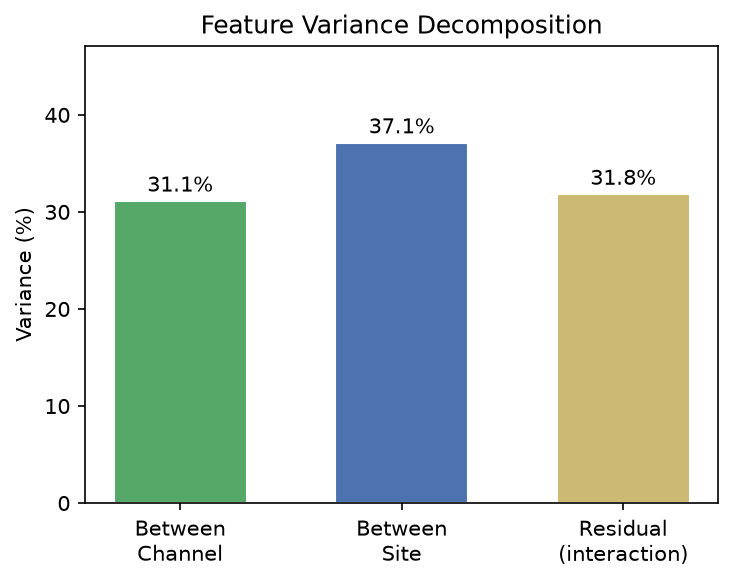
\includegraphics[width=\columnwidth]{figures/variance_decomp.png}
    \caption{Variance decomposition of the cached DINOv3 tokens on plate BR00116991: between-channel, between-site and residual components.}
    \label{fig:variance}
\end{figure}

\begin{figure}[t]
    \centering
    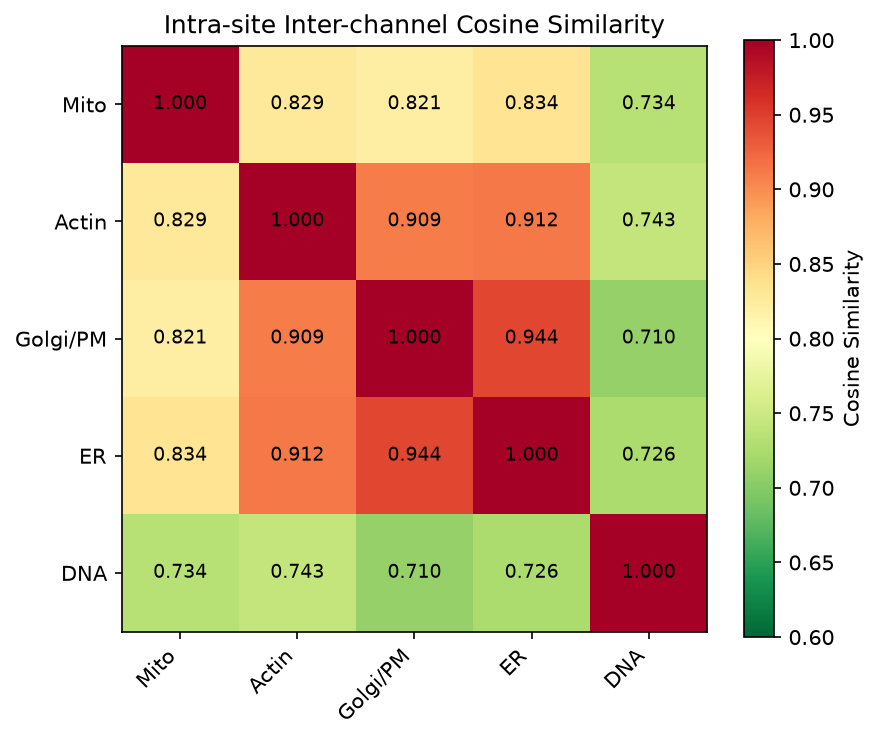
\includegraphics[width=\columnwidth]{figures/channel_similarity.png}
    \caption{Mean cosine similarity between fluorescence channels in the cached token space. The DNA channel is the most distinct.}
    \label{fig:channelsim}
\end{figure}

\begin{figure}[t]
    \centering
    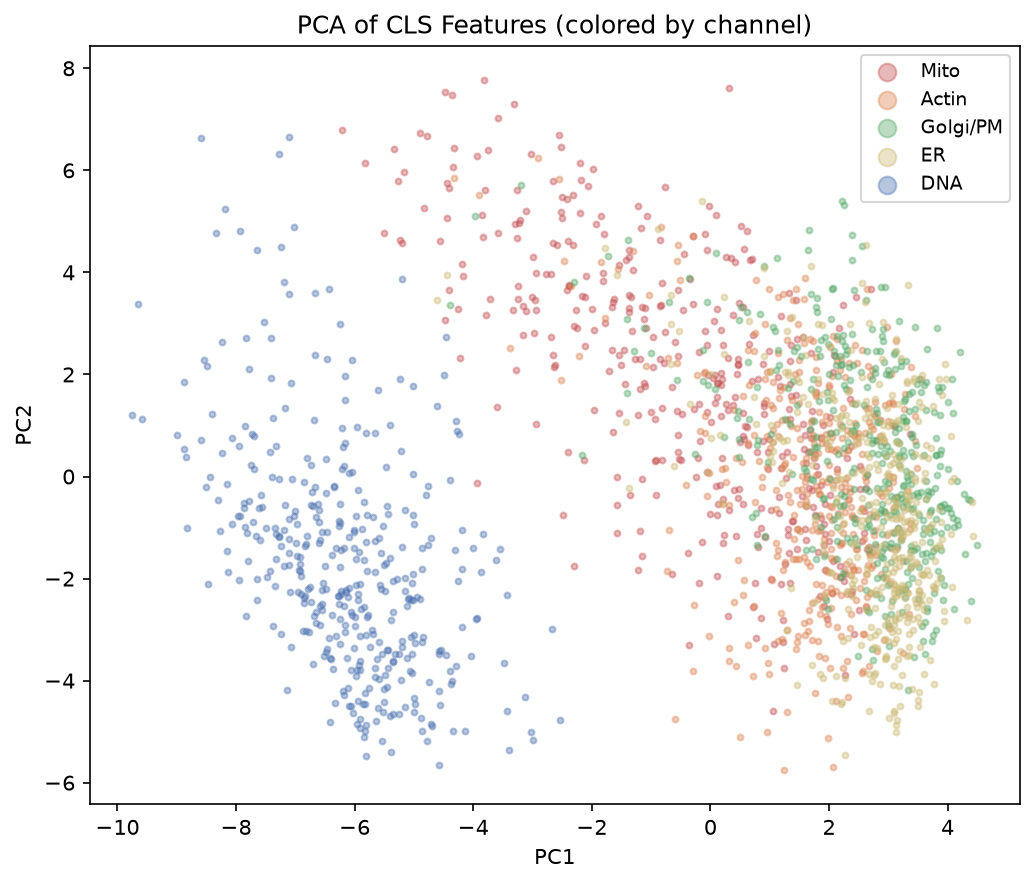
\includegraphics[width=\columnwidth]{figures/pca_channels.png}
    \caption{First two principal components of the cached 1024-d channel tokens, colored by fluorescence channel.}
    \label{fig:pca}
\end{figure}

\subsection{Cost}

For the no-offset ablation runs, \texttt{metrics.csv} records about four seconds for the training-loop phase of an epoch with 55 steps at batch size 256 on the RTX 5080. This excludes validation, data loading outside the timer and the offset-refresh pass used by offset variants, so it is not an end-to-end run-time measurement. Both backbones stay frozen; the trainable components are the CrossChannelFormer, two projection heads and one logit-scale scalar.

\section{Conclusion}
\label{sec:conclusion}

MorphoCLIP maps Cell Painting wells and text descriptions of perturbations into a 512-dimensional space with about 14M trainable parameters on top of two frozen backbones. One model handles compounds, CRISPR knockouts and ORF overexpressions. At one seed, perturbation-level Recall@10 is about 39\% in both directions on validation and 37 to 44\% on test, against analytic chance rates of 10 to 12\%. Separate stochastic benchmark runs show numerically comparable compound replicability fractions for MorphoCLIP and the released CellCLIP checkpoint but do not support a ranking. The base model's four-track mean compound target-matching fraction lies within the published CellProfiler range, although one track is above it.

Gene-aware soft labels, the replicate alignment loss and condition-relative plate offsets each change validation retrieval by only a few perturbations, and the test split reorders them. These retrieval differences are unresolved without repeated seeds. The replicate loss does increase deterministic replicability mAP on every track, from pooled 0.298 to 0.343, while the combined run reaches 0.369. This result is partly definitional because the loss directly optimizes replicate proximity. The in-batch plate correction degrades retrieval because the plate mean carries condition information named by the prompt; the condition-relative offset avoids that degradation but shows no consistent retrieval or benchmark-mAP improvement at this seed count.

Gene--compound fraction retrieved is at or near zero for every model: at most three admitted pairs pass the stochastic significance gate in any run. We have no positive cross-modality result.

\subsection{Limitations and Future Work}

Every retrieval number in this paper is from one seed. Repeated seeds are needed for the control, replicate-loss and combined runs. Fraction retrieved on the standard benchmark varies between runs of the same code, so those values are descriptive. We did not rerun CellProfiler, and the CellCLIP row comes from a separate run with a different export path and a batch-correction step ours lacks. Because the replicate loss directly optimizes the replicability task, evidence that the embedding is more informative requires a task outside that objective; target matching does not provide such evidence here.

On cross-modality, one concrete lead is the choice of gene annotation. Training soft labels use each compound's primary target (160 distinct genes) while the benchmark's gene--compound track uses the full target list (758 distinct genes, off-targets included). Aligning the two, or training on the wider list, is a one-line change we have not measured. A second lead is prompt content: whether the SMILES string and gene-function text carry signal through BioClinical ModernBERT, or are inert, can be tested by ablating them out of the templates. Beyond CPJUMP1, the full JUMP corpus of about 140,000 perturbations across many sites and cell lines is the setting in which a text-supervised model would have to prove that its embeddings transfer.

We release the code, configs, split manifests and the evaluation harness with the paper.


\bibliographystyle{IEEEtran}
\bibliography{references}

\end{document}
